%! Author = Raffaele
%! Date = 11/01/2024

\thispagestyle{headings}
\newpage
\section{Il Game Handler}\label{sec:game-handler}

\begin{figure}
    \centering
    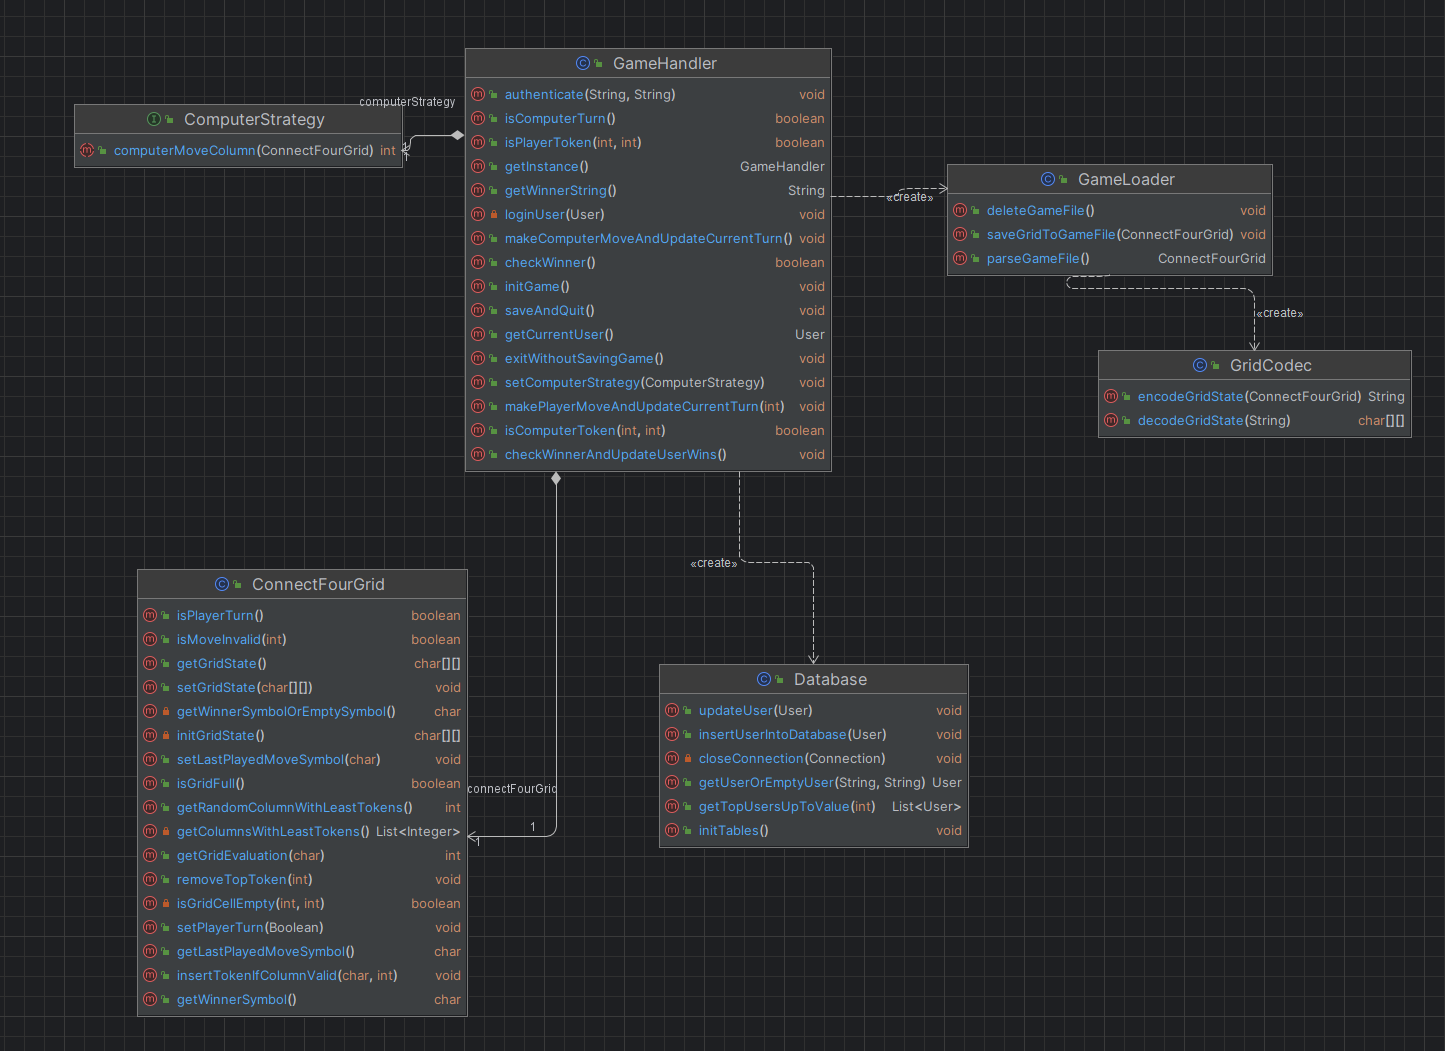
\includegraphics[scale=0.4]{img/gamehandler-uml}
    \caption{Diagramma UML della classe GameHandler}
    \label{fig:gamehandler-uml}
\end{figure}

GameHandler è la \textit{de facto} classe principale dell'applicazione. \\
La funzione della classe è quello di definire un insieme di metodi che permettano di gestire lo scorrimento della
partita senza esporre l'oggetto griglia (definito dalla classe \textit{ConnectFourGrid}). \\
Il Game Handler utilizza la classe ausiliaria \textit{GameLoader} per delegare la gestione dei file,
che a sua volta delega la codifica e decodifica della griglia alla classe \textit{GridCodec}. \\
\textit{GridCodec} permette di trasformare la rappresentazione della griglia di gioco nel programma, che utilizza
un array di caratteri, in una stringa salvata su file, e di effettuare l'operazione inversa, al fine di permettere
il salvataggio di una partita in corso e la successiva ripresa. \\
Il Game Handler mantiene una reference ad un oggetto che implementa l'interfaccia \textit{ComputerStrategy} che
permette di ottenere una mossa da parte del computer quando richiesto. \\
Infine, si interfaccia con la classe \textit{Database} per aggiornare l'utente attualmente autenticato. \\
GameHandler implementa il Design Pattern \textbf{Singleton}\cite{GoF} in quanto vogliamo esista solo un Gamehandler, e che questi
sia globalmente accessibile. \\

Si potrebbe pensare che questa classe violi il \textit{Single Responsibility Principle}, tuttavia tutto ciò che fa di
concreto è indirizzare il proseguimento della partita richiamando metodi di altre classi, le implementazioni vere
e proprie sono incapsulate in tali classi e pertanto totalmente disaccoppiate.

\newpage
\section{La griglia}\label{sec:la-griglia}

\begin{figure}
    \centering
    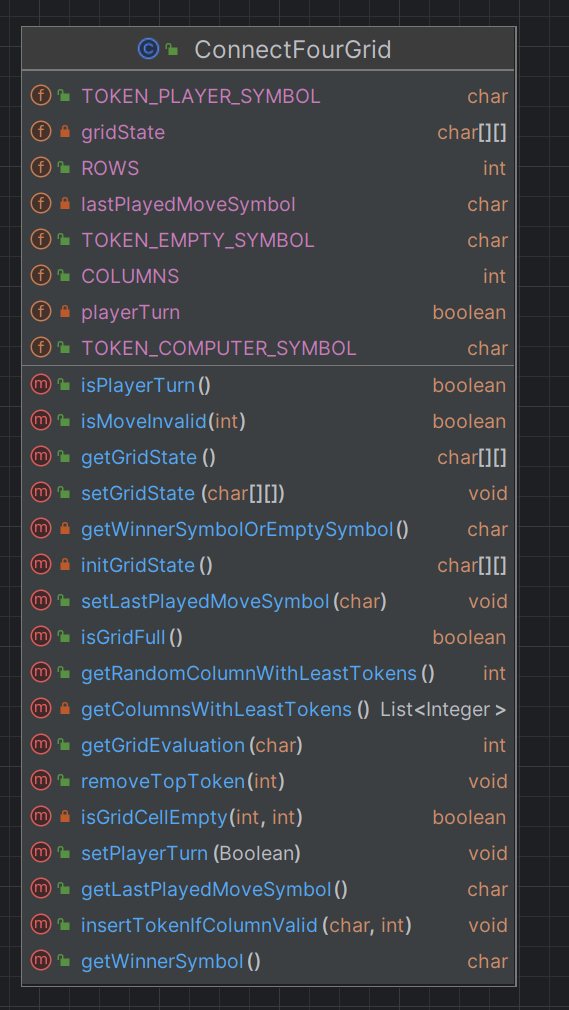
\includegraphics[scale=0.4]{img/connectfourgrid-uml}
    \caption{Diagramma UML della classe ConnectFourGrid}
    \label{fig:connectfourgrid-uml}
\end{figure}

La class \textit{ConnectFourGrid} incapsula il comportamento della griglia rappresentata da un array bidimensionale
di caratteri, ed espone metodi per intervenire direttamente sulle pedine presenti nella griglia e controllare la
situazione all'interno di essa. \\

\begin{figure}
    \begin{verbatim}
    public void insertTokenIfColumnValid(char tokenSymbol,
                                        int column) {
        if (isMoveInvalid(column)) {
            return;
        }
        for (int i = 0; i < ROWS; i++) {
            if (i == ROWS - 1) {
                if (isGridCellEmpty(i, column)) {
                    gridState[i][column] = tokenSymbol;
                    this.lastPlayedMoveSymbol = tokenSymbol;
                }
            } else if (!isGridCellEmpty(i + 1, column) &&
                        isGridCellEmpty(i, column)) {
                gridState[i][column] = tokenSymbol;
                this.lastPlayedMoveSymbol = tokenSymbol;
            }
        }
    }
    \end{verbatim}
    \caption{Metodo utilizzato dalla griglia per inserire una pedina}
    \label{fig:code-grid1}
\end{figure}

Il metodo insertTokenIfColumnValid controlla prima se la colonna scelta non è attualmente piena, e se possibile
scorre la colonna fino a trovare lo spazio libero più in basso per inserire una pedina.

\begin{figure}
    \begin{verbatim}
    public int getRandomColumnWithLeastTokens() {
        List<Integer> values = getColumnsWithLeastTokens();
        Random r = new Random();
        int index = r.nextInt(values.size());
        return values.get(index);
    }
    \end{verbatim}
    \caption{Metodo utilizzato per selezionare una colonna a caso tra quelle con meno pedine}
    \label{fig:code-grid2}
\end{figure}


Il metodo getRandomColumnWithLeastTokens sfrutta la funzione ausiliaria \textit{getColumnsWithLeastTokens} per
ritornare una colonna casuale tra quelle che attualmente contengono il numero minore di pedine.

\newpage
\section{ComputerStrategy}\label{sec:computerstrategy}

\begin{figure}
    \centering
    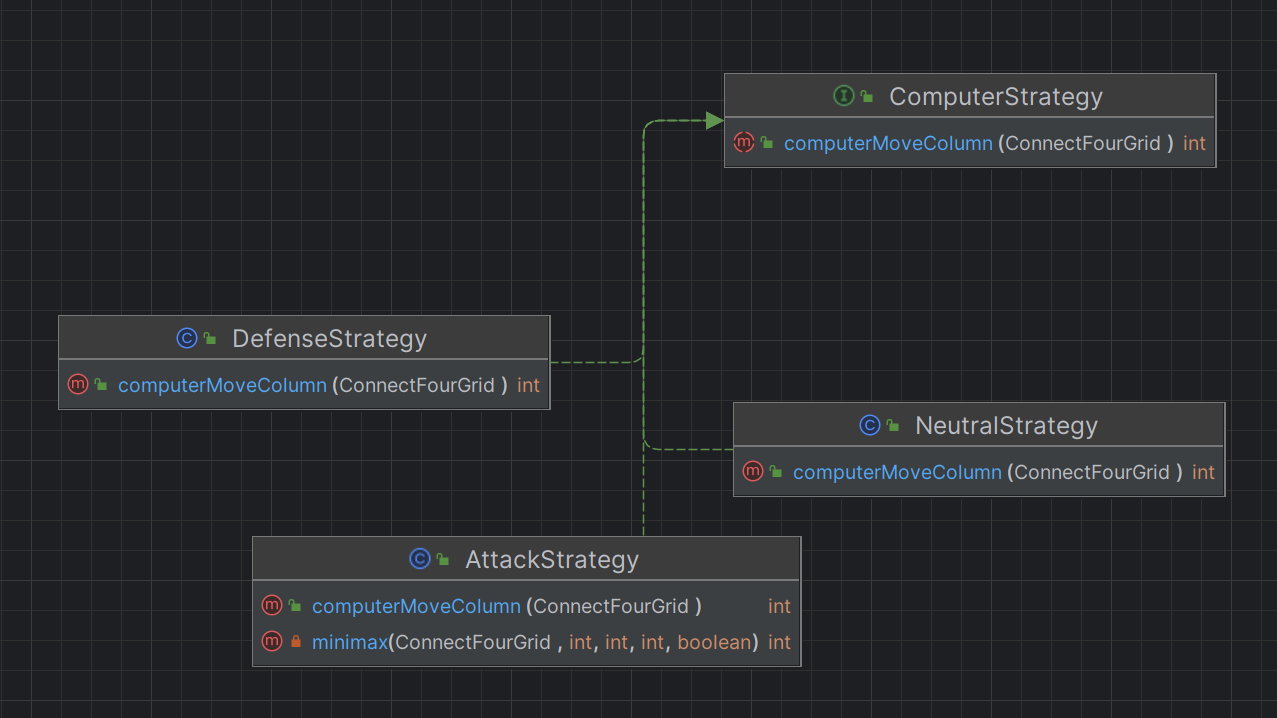
\includegraphics[scale=0.4]{img/strategy-uml}
    \caption{Diagramma UML dell'interfaccia ComputerStrategy}
    \label{fig:strategy-uml}
\end{figure}

L'interfaccia \textit{ComputerStrategy} è utilizzata per implementare il Design Pattern \textbf{Strategy}~\cite{GoF},
permettendo di incapsulare i diversi algoritmi utilizzati per la scelta da parte del computer di una mossa. \\
Strategy rende possibile cambiare l'algoritmo a run-time, e diventa estremamente facile aggiungere nuove modalità
di gioco semplicemente creando nuove classi che implementano tale interfaccia.
ComputerStrategy espone un unico metodo chiamato \textit{computerMoveColumn} che ritorna la colonna dove inserire
la pedina del computer. \\
L'algoritmo di scelta della colonna è così totalmente disaccoppiato dalla griglia e dal GameHandler. \\

\subsection{AttackStrategy}\label{subsec:attackstrategy}

La classe \textbf{AttackStrategy} utilizza l'algoritmo \textbf{Minimax con Alpha-beta pruning}\cite{Wiki} per scegliere la mossa.
L'algoritmo viene implementato in questo modo: \\
\begin{itemize}
    \item Si controllano tutte le colonne e vengono inserite in un array di interi dove l'indice nell'array indica
    l'indice della colonna stessa e il valore corrispondente a quell'indice indica la valutazione della mossa stessa.
    A una mossa invalida viene associato il valore di \textit{Integer.MIN\_VALUE} in modo che non possa essere scelta.
    \item L'algoritmo di \textbf{minimax} viene utilizzato per dare una valutazione a ogni possibile mossa.
    (Continua sotto)
    \item Alla fine, le mosse con la valutazione più alta vengono inserite in un ArrayList.
    Se vi è più di una mossa migliore, ne viene selezionata una casualmente.
\end{itemize}

L'algoritmo \textbf{Minimax} è un algoritmo ricorsivo che si basa sull'idea di \textit{minimizzare la massima perdita}.
Applicato al gioco \textit{Forza quattro} la massima perdita indica la perdita di una partita, ovvero quando
l'avversario è in grado di concatenare quattro delle proprie pedine. \\
In generale, l'algoritmo funziona alternando i turni di inserimento delle pedine, e facendo finta di inserirle.
Questo finto inserimento serve per valutare la situazione della griglia per controllare se vi è o meno un vincitore, e
associare un punteggio alla mossa in questione. \\
L'alternanza dei turni permette a ogni ricorsione di valutare la miglior mossa dal punto di vista del turno corrente.
Poiché l'algoritmo viene eseguito inizialmente dal computer, se la posizione della griglia indica una vittoria
del giocatore, viene associato uno punteggio alla mossa molto basso, o più semplicemente negativo, viceversa una
vittoria del computer associa alla mossa un punteggio maggiore. \\
\\
La complessità dell'algoritmo Minimax è proporzionale al numero di nodi generati dall'albero di ricorsione, ovvero $O(b^d)$ \\
dove \textit{b} indica il numero di mosse possibili a ogni turno, e \textit{d} la profondità della ricerca. \\
Tuttavia le prestazioni dell'algoritmo possono essere migliorate notevolmente applicando il cosidetto
\textbf{Alpha-beta pruning}, che è una miglioria all'algoritmo base, in quanto evita di continuare a esplorare una
mossa se almeno una sotto-mossa è stata trovata che renda quella mossa peggiore di un'altra già trovata.
Per fare ciò l'algoritmo utilizza due valori chiamati \textit{Alfa} e \textit{beta} che mantengono rispettivamente
il valore minimo che il giocatore \("\)massimizzante\("\) è assicurato di avere da una mossa, e il valore massimo che
il giocatore \("\)minimizzante\("\) può ottenere da quella mossa. \\
La ricerca della mossa corrente viene fermata nel momento in cui $alpha \geq beta$. \\
Nel caso peggiore, l'Alpha-beta pruning ha le stesse prestazioni dell'algoritmo minimax classico, tuttavia nel caso
medio le prestazioni si avvicinano di più a $O(\sqrt {b^d})$. \\
Per rendere l'idea, ho deciso di effettuare un piccolo \("\)benchmark\("\) dell'algoritmo minimax con e senza
alpha-beta pruning, con tutti gli altri fattori lasciati immutati, i risultati sono visibili nella tabella~\ref{fig:benchmark}.

\begin{figure}
    \begin{center}
        \begin{tabular}{||c c c||}
            \hline
            Profondità & Minimax & Alpha-beta\\ [0.5ex]
            \hline\hline
            2 & 0.9 ms & 0.9 ms \\
            \hline
            3 & 7.0 ms & 2.5 ms \\
            \hline
            4 & 31.1 ms & 8.1 ms \\
            \hline
            5 & 56.4 ms & 19.8 ms \\
            \hline
            6 & 109.6 ms & 31.7 ms \\
            \hline
            7 & 341.2 ms & 44.1 ms \\
            \hline
            8 & 1.5 s & 53.2 ms \\
            \hline
            9 & 10.4 s & 100.0 ms \\
            \hline
            10 & 1 min & 159.3 ms \\
            \hline
            11 & 7.4 min & 387 ms \\
            \hline
            12 & & 1.2 s \\
            \hline
            13 & & 6.1 s \\
            \hline
            14 & & 21.2 s \\
            \hline
            15 & & 2 min \\
            \hline
            16 & & 6.5 min \\ [1ex]
            \hline
        \end{tabular}
    \end{center}
    \caption{Tabella che indica i tempi di esecuzione in relazione alla profondità}
    \label{fig:benchmark}
\end{figure}

L'implementazione della funzione di minimax è mostrata nella figura~\ref{fig:minimax}. \\
Nell'applicazione ho deciso di optare per una ricerca base di profondità 10. \\

\begin{figure}
    \centering
    \begin{verbatim}
        private int minimax(ConnectFourGrid connectFourGrid, int depth,
                            int alpha, int beta, boolean isComputerTurn) {
        if(depth <= 0) {
            return 0;
        }
        int currentGridEvaluation = connectFourGrid.getGridEvaluation(
                                    connectFourGrid.TOKEN_COMPUTER_SYMBOL);
        if(currentGridEvaluation == 1) {
            return depth;
        } else if(currentGridEvaluation == -1) {
            return -depth;
        } else if(connectFourGrid.isGridFull()) {
            return 0;
        }

        if(isComputerTurn) {
            int maxValue = Integer.MIN_VALUE;
            for(int j = 0; j < connectFourGrid.COLUMNS; j++) {
                if(connectFourGrid.isMoveInvalid(j)) { continue; }
                connectFourGrid.insertTokenIfColumnValid(
                                connectFourGrid.TOKEN_COMPUTER_SYMBOL, j);
                maxValue = Math.max(maxValue,
                            minimax(connectFourGrid, depth - 1,
                                            alpha, beta, false));
                connectFourGrid.removeTopToken(j);
                alpha = Math.max(alpha, maxValue);
                if(alpha >= beta) {
                   break;
                }
            }
            return maxValue;
        } else {
            int minValue = Integer.MAX_VALUE;
            for(int j = 0; j < connectFourGrid.COLUMNS; j++) {
                if(connectFourGrid.isMoveInvalid(j)) { continue; }
                connectFourGrid.insertTokenIfColumnValid(
                                connectFourGrid.TOKEN_PLAYER_SYMBOL, j);
                minValue = Math.min(minValue,
                            minimax(connectFourGrid, depth - 1,
                                            alpha, beta, true));
                connectFourGrid.removeTopToken(j);
                beta = Math.min(beta, minValue);
                if(alpha >= beta) {
                    break;
                }
            }
            return minValue;
        }
    }
    \end{verbatim}
    \caption{Algoritmo Minimax con Alpha-beta pruning}
    \label{fig:minimax}
\end{figure}

\newpage
\subsection{DefenseStrategy}\label{subsec:defensestrategy}

La strategia \textit{Difesa} cerca semplicemente di bloccare le pedine dell'utente, per fare ciò l'algoritmo controlla
tutte le colonne, tutte le righe ed entrambe le direzioni diagonali (ascendente e discendente) e mantiene traccia
del numero di pedine dell'utente in quella direzione all'interno di una \textit{Hash Table} implementata come
una \textit{HashMap} di Java. \\
La hash table identifica ogni direzione con una stringa ottenuta concatenando il tipo di direzione (h - horizontal,
v - vertical, ad - ascending diagonal, dd - descending diagonal) con il numero di colonna da cui è iniziato il contatore
delle pedine. \\
In questo modo la HashMap contiene informazioni sul numero di pedine per ogni direzione, ma ogni direzione conserva
implicitamente anche la colonna dove eventualmente inserire la pedina del computer. \\
La HashMap viene quindi ordinata per valori, e la chiave relativa al valore più alto viene riconvertita in un numero
di colonna che viene ritornato. \\
Se ci sono più chiavi con lo stesso valore, viene ritornata la prima. \\
Se le chiave da ritornare è 0 o 1, viene invece ritornato il numero di una colonna a caso tra quelle contenenti
meno pedine, utilizzando il metodo \textit{getColumnsWithLeastTokens} della classe \textit{ConnectFourGrid}. \\
L'implementazione della modalità difesa è visibile nel codice in figura~\ref{fig:defense-strategy}.

\begin{figure}
    \centering
    \begin{verbatim}
        public int computerMoveColumn(ConnectFourGrid connectFourGrid) {
        char symbolToCount = connectFourGrid.TOKEN_PLAYER_SYMBOL;
        Map<String, Integer> playableColumnsWithMostConnectedTokens
                                = new HashMap<>();
        // horizontal
        for(int i = 0; i < connectFourGrid.ROWS; i++) {
            for(int j = 0; j < connectFourGrid.COLUMNS - 3; j++) {
                if(connectFourGrid.isMoveInvalid(j)) {
                    continue;
                }
                int currentCount = 0;
                for(int k = 0; k <= 3; k++) {
                    if(connectFourGrid.getGridState()[i][j + k]
                            == symbolToCount) {
                        currentCount++;
                    }
                }
                playableColumnsWithMostConnectedTokens
                    .put("h"+j, currentCount);
            }
        }
        // stessa operazione per le altre direzioni
        // ...
        // codice omesso per semplicità

        String highestKey = Collections.max(
                playableColumnsWithMostConnectedTokens.entrySet(),
                Map.Entry.comparingByValue()).getKey();

        int value = playableColumnsWithMostConnectedTokens
                        .get(highestKey);
        // regex per togliere i caratteri non-cifre
        int column = Integer.parseInt(highestKey
                            .replaceAll("[^\\d.]", ""));
        if(value == 0 ||
           value == 1 ||
            connectFourGrid.isMoveInvalid(column)) {
            return connectFourGrid.getRandomColumnWithLeastTokens();
        }
        return column;
    }
    \end{verbatim}
    \caption{Algoritmo che implementa la modalità difesa descritta}
    \label{fig:defense-strategy}
\end{figure}

\newpage
\subsection{NeutralStrategy}\label{subsec:neutralstrategy}

La strategia \textit{Neutrale} sceglie casualmente tra la strategia \textit{Difesa} e la strategia \textit{Attacco} per
selezionare una mossa. \\
La scelta casuale è ottenuta attraverso il metodo \textit{nextBoolean()} della classe \textit{java.util.Random}. \\


\newpage
\section{Gestione del Database}\label{sec:gestione-del-database}

\begin{figure}
    \centering
    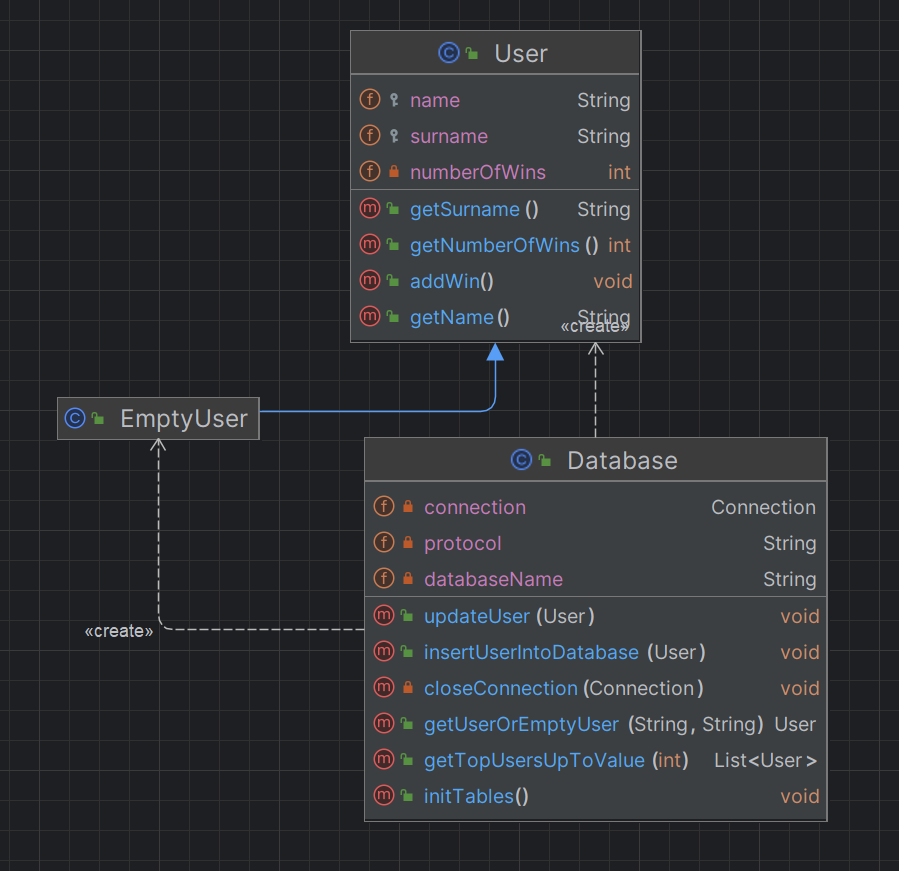
\includegraphics[scale=0.5]{img/database-uml}
    \caption{Diagramma UML della classe Database}
    \label{fig:database-uml}
\end{figure}

La classe Database incapsula l'interazione con il Database SQLite, esponendo dei metodi che permettono di agire con
la classe \textit{User} traducendo le operazioni effettuate in operazioni sul database, e viceversa. \\
Per esempio, la figura~\ref{fig:db1} mostra il metodo utilizzato per inserire un utente nella tabella utenti. \\

\begin{figure}
    \begin{verbatim}
    public void insertUserIntoDatabase(User user) {
        try {
            connection = DriverManager
                         .getConnection(protocol + databaseName);
            String sql = "INSERT INTO users (name, surname, wins)"
                    + " VALUES(?, ?, ?)";
            PreparedStatement statement = connection.prepareStatement(sql);
            statement.setString(1, user.getName());
            statement.setString(2, user.getSurname());
            statement.setInt(3, user.getNumberOfWins());
            statement.execute();
        } catch (SQLException e) {
            System.out.println(e.getMessage());
        } finally {
            closeConnection(connection);
        }
    }
    \end{verbatim}
    \caption{Metodo utilizzato per inserire un oggetto della classe Utente all'interno del database}
    \label{fig:db1}
\end{figure}

Tutte le operazioni sul database si compongono delle seguenti fasi:
\begin{itemize}
    \item Creazione di una connessione tramite il metodo\\
    \textit{DriverManager.getConnection(protocol + databaseName)} dove \textit{protocol} e \textit{databaseName}
    sono dei campi della classe Database che indicano rispettivamente il driver da utilizzare per accedere
    al database SQLite e il nome del file che contiene il database.
    \item Creazione ed esecuzione di uno statement SQL, solitamente un \textit{PreparedStatement}.
    \item Chiusura della connessione, effettuata in questo caso attraverso il metodo ausiliario \textit{closeConnection}
    che si occupa di effettuare il \textit{try/catch} sull'operazione di close, utilizzato principalmente per leggibilità.
\end{itemize}

Infine, la classe EmptyUser serve per gestire il caso in cui un utente sia inesistente nel database,
per evitare di ritornare \textit{null}\cite{CleanCode} dalla funzione che converte un utente nel database in un oggetto \textit{User}.
